%%%%%%%%%%%%%%%%%%%%%%%%%%%%%%%%%%%%%%%%%%%%%%%%%%%%%%%%%%%%%%%%%%%%%%%%%%%%%%%%
% IEEE RAS conference template (ieeeconf.cls, https://ras.papercept.net/conferences/support/tex.php)
% Build:  pdflatex paper && pdflatex paper     (figures are in ./figures; produced by report.ipynb)
%%%%%%%%%%%%%%%%%%%%%%%%%%%%%%%%%%%%%%%%%%%%%%%%%%%%%%%%%%%%%%%%%%%%%%%%%%%%%%%%

\documentclass[letterpaper, 10 pt, conference]{ieeeconf}

\IEEEoverridecommandlockouts
\overrideIEEEmargins

\usepackage{graphicx}
\usepackage{amsmath}
\usepackage{amssymb}
\usepackage{booktabs}
\usepackage{url}

\title{\LARGE \bf
Camera Failure and Recovery in Three Camera-Only 3D Detectors:\\
An Event-Based Study on nuScenes
}

% TODO: replace the placeholder names and affiliation before submission.
\author{Author One$^{1}$, Author Two$^{1}$, Author Three$^{1}$, and Author Four$^{1}$% <-this % stops a space
\thanks{$^{1}$The authors are with the ROB535 course team, [Department, University], [City, Country]
        {\tt\small \{author1, author2, author3, author4\}@example.edu}}%
}

\begin{document}

\maketitle
\thispagestyle{empty}
\pagestyle{empty}

%%%%%%%%%%%%%%%%%%%%%%%%%%%%%%%%%%%%%%%%%%%%%%%%%%%%%%%%%%%%%%%%%%%%%%%%%%%%%%%%
\begin{abstract}
Multi-camera 3D detectors are benchmarked on clean data, yet a camera stream can drop out in deployment, and a temporal detector may carry
contaminated state when it returns. We study how three released camera-only detectors with different temporal memory (BEVFormer: recurrent BEV
features; StreamPETR: propagated object queries; SparseBEV: a window of eight keyframes) lose and regain detection after a front-camera outage on nuScenes.
Our contribution is an event-based protocol: one physical outage schedule shared by all models, black-image injection before preprocessing with an
audit of every consumed image, per-model operating points fixed on separate pilot scenes, frozen damage and recovery rules that keep right-censored events apart from
failures, and a paired scene bootstrap. On 150 validation scenes all models lose 9--22 points of front-region recall during the outage, and the pooled loss is back inside
a 5-point margin at the first bin after restoration, except SparseBEV and StreamPETR after 2\,s outages (7 points). From 0.5\,s on the pooled loss stays within 3 points of zero, although
SparseBEV's window holds black frames for about 3.5\,s. Failure analysis shows that objects still missed after restoration grow with outage length
(up to 21\% for StreamPETR) and that precision drops for two of the three models. Code is linked in Section~VII.
\end{abstract}

%%%%%%%%%%%%%%%%%%%%%%%%%%%%%%%%%%%%%%%%%%%%%%%%%%%%%%%%%%%%%%%%%%%%%%%%%%%%%%%%
\section{INTRODUCTION}

Camera-only 3D detection is a core perception component for low-cost autonomous driving, and the strongest recent systems are temporal: they
reuse past frames to resolve depth, motion and occlusion. That reuse creates a failure mode that clean benchmarks do not
exercise. If a camera stream goes dark because of a hardware fault or a communication loss, the detector is fed blank input; when the stream returns, features,
queries or cached states built from the blank frames may still be in memory. A safety-relevant question follows: \emph{after a front-camera outage,
how quickly does detection recover, and how much does the answer depend on the model's temporal history?}

Standard robustness benchmarks corrupt every frame of a scene and report one aggregate score \cite{dong2023,xie2023,zhu2023}.
Such scores measure degradation \emph{under} a condition, not behavior \emph{across a transition}: they cannot show when degradation starts, how large it is
during a bounded outage, or when it ends. We therefore analyze three existing, pretrained detectors rather than propose a new one; our novelty is the evaluation methodology.
\begin{itemize}
\item An \textbf{event-based outage protocol}: every model sees the same physical outage (scenes, start times, durations), black
images are injected before resizing and normalization, and every consumed image is audited.
\item \textbf{Recovery metrics} on the same eligible objects for paired clean and outage runs, with frozen damage and recovery rules, per-model
operating points calibrated on separate scenes, and explicit right-censoring of events whose follow-up is incomplete.
\item A \textbf{quantitative and failure-mode analysis} on 150 nuScenes validation scenes with paired scene-bootstrap intervals and state-isolation controls.
\end{itemize}

%%%%%%%%%%%%%%%%%%%%%%%%%%%%%%%%%%%%%%%%%%%%%%%%%%%%%%%%%%%%%%%%%%%%%%%%%%%%%%%%
\section{RELATED WORK}

\textbf{Multi-camera 3D detection.} DETR3D \cite{detr3d} and PETR \cite{petr} lift multi-view images to 3D with queries or position embeddings.
Temporal reasoning followed in several forms: BEVDet4D \cite{bevdet4d} fuses aligned BEV features of past frames; BEVFormer \cite{bevformer} propagates a recurrent BEV
representation with ego-motion alignment; StreamPETR \cite{streampetr} keeps an object-centric memory of propagated queries; SparseBEV \cite{sparsebev} samples features from
a finite window of past frames. We study one representative of each of the last three, which differ in the property that matters here:
how long information from one input frame can persist.

\textbf{Robustness benchmarks.} Common-corruption benchmarks \cite{hendrycks2019} were extended to 3D detection: nuScenes-C \cite{dong2023} and RoboBEV \cite{xie2023}
corrupt every camera frame, and Zhu~\emph{et al.}~\cite{zhu2023} compare BEV and non-BEV detectors under natural and adversarial perturbations. These studies treat a
corruption as a constant property of a whole sequence.

\textbf{Sensor failure.} MetaBEV \cite{ge2023} and the LiDAR--camera benchmark of Yu~\emph{et al.}~\cite{yu2023} study missing or corrupted sensors in fusion models,
and BEVFusion \cite{bevfusion} lets one modality compensate for another. A camera-only system has no second modality, and the \emph{transient}
nature of a dropout and the role of temporal memory after it ends have received little attention. We address that gap on nuScenes \cite{nuscenes}.

%%%%%%%%%%%%%%%%%%%%%%%%%%%%%%%%%%%%%%%%%%%%%%%%%%%%%%%%%%%%%%%%%%%%%%%%%%%%%%%%
\section{APPROACH}

\subsection{Detectors and temporal state}
We use released checkpoints without retraining: \textbf{BEVFormer-tiny} (R50), whose recurrent BEV is aligned by CAN-bus ego motion;
\textbf{StreamPETR} (R50, 704\,px) with a propagated query memory; and \textbf{SparseBEV} (R50, 704$\times$256), whose temporal input is the current keyframe plus
seven previous keyframes and whose feature cache is keyed by file name. Each runs in its own project runner (batch one, TF32 off, deterministic cuDNN); repeated clean runs are
bit-identical, and each clean baseline reproduces its released score within $\pm 0.010$ NDS (0.3545, 0.537, 0.556; a gate declared before the results; SparseBEV is gated on NDS
only, as its release publishes no mAP).

\subsection{Outage protocol}
Each of the 150 nuScenes validation scenes receives one outage (Fig.~\ref{fig:protocol}) that starts at the CAM\_FRONT sensor timestamp of keyframe six, leaving six clean keyframes,
and lasts $d\in\{0.5,1,2\}$\,s. Every CAM\_FRONT image whose sensor timestamp lies in the half-open window of length $d$ from the start is replaced by an all-black image
\emph{before} resizing and normalization, so the camera is dark rather than the features. A sample may use images up to 50\,ms later than its own timestamp (a causal allowance). The schedule is frozen,
identical across the three projects, and never changed from detection outcomes. Each consumed image is logged with path, timestamp and pixel hash before and after corruption; the black counts
(168, 326, 635 on validation) match an independent recount.

\begin{figure}[t]
\centering
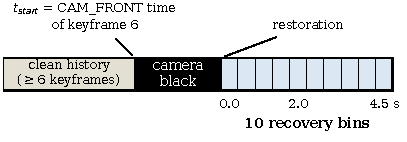
\includegraphics[width=0.92\columnwidth]{figures/fig_protocol.pdf}
\caption{Outage protocol shared by all models: the front camera is black for $d$ seconds from keyframe six; recovery is followed in ten 0.5\,s bins.}
\label{fig:protocol}
\end{figure}

\subsection{Event-based recovery metrics}
\textbf{Region and operating point.} Evaluation is restricted to the region the outage affects: ground-truth objects with centers in the CAM\_FRONT view within 50\,m, matched to predictions
one-to-one by score within 2\,m on a single ego ground plane. Each model gets one score threshold (SparseBEV 0.542, StreamPETR 0.758, BEVFormer 0.879), calibrated on ten \emph{pilot}
training-split scenes to the highest precision subject to recall $\ge 0.30$ and $\ge 100$ region predictions, and fixed before any validation outcome was inspected.

\textbf{Loss.} For a phase (during the outage, or a post-restoration bin) the pooled loss is $L=R_{\text{clean}}-R_{\text{outage}}$, with both recalls on the same eligible objects of the paired runs.
Post-restoration samples are assigned one-to-one to bins 0.0--4.5\,s ($\pm$0.25\,s).

\textbf{Events and censoring.} An event is a (scene, duration) pair, \emph{damaged} if its loss during the outage exceeds 0.05 with at least five eligible objects. Recovery onset is the first
post-restoration bin with $L\le 0.05$ whose adjacent next bin also qualifies. A missing or insufficient bin breaks the pair, so an event without a confirmable onset is
\emph{right-censored} (unknown), not a failure, unless every follow-up pair was usable.

\subsection{Uncertainty and controls}
Intervals are percentile 95\% intervals of a paired complete-scene bootstrap ($B=10{,}000$): scenes are resampled with replacement and \emph{one} weight matrix is shared by all models and durations, preserving the
clean/outage pairing, within-scene dependence and cross-model pairing. Aggregate degradation is declared only if the pooled loss exceeds 0.05 and its interval excludes zero.
Controls: the aggregate tables were rebuilt independently from per-sample match records (64,350 cells per model, exact agreement); a run-integrity gate stops the analysis if any of the 30 runs fails its checks;
a pilot outage re-run from its saved configuration reproduced predictions and audit records bit-for-bit; and every SparseBEV sample whose window holds no black frame equals the clean run (the window clears about 3.5\,s after restoration).

%%%%%%%%%%%%%%%%%%%%%%%%%%%%%%%%%%%%%%%%%%%%%%%%%%%%%%%%%%%%%%%%%%%%%%%%%%%%%%%%
\section{EXPERIMENTAL RESULTS}

\subsection{Loss during the outage}
All three detectors lose front-region recall while the camera is black (Table~\ref{tab:main}, Fig.~\ref{fig:results}a). The pooled loss grows with duration, from
0.09--0.17 at 0.5\,s to 0.15--0.22 at 2\,s, and every 95\% interval excludes zero. Relative to clean recall, StreamPETR loses 29--48\% of what it detects, SparseBEV 40--60\% and
BEVFormer 59--79\%. StreamPETR loses least at every duration. This ordering is descriptive: the systems differ in clean recall at their operating points (0.26--0.36), resolution, pretraining, query count and history, so it is not
evidence about any one architectural choice.

\begin{table}[t]
\caption{Pooled recall loss during the outage and at 0.0\,s after restoration, per-event damage rate (events with $\ge$5 objects) and share of missed objects detected again; 95\% intervals in parentheses.}
\label{tab:main}
\centering
\scriptsize
\setlength{\tabcolsep}{2.2pt}
\begin{tabular}{llcccc}
\toprule
Model & $d$ & Loss during & @0.0\,s & Damage rate & Re-det. \\
\midrule
SparseBEV  & 0.5 & 0.145 (.119--.170) & 0.023 & 0.66 (.54--.77) & 0.95 \\
           & 1   & 0.171 (.143--.199) & 0.040 & 0.71 (.62--.80) & 0.89 \\
           & 2   & 0.213 (.187--.238) & 0.072 & 0.74 (.67--.82) & 0.85 \\
StreamPETR & 0.5 & 0.093 (.068--.116) & 0.019 & 0.49 (.37--.60) & 0.87 \\
           & 1   & 0.118 (.096--.140) & 0.037 & 0.57 (.47--.66) & 0.80 \\
           & 2   & 0.149 (.125--.173) & 0.074 & 0.63 (.55--.72) & 0.70 \\
BEVFormer  & 0.5 & 0.168 (.141--.195) & 0.014 & 0.79 (.68--.88) & 0.89 \\
           & 1   & 0.194 (.170--.221) & 0.027 & 0.79 (.70--.86) & 0.88 \\
           & 2   & 0.224 (.198--.253) & 0.030 & 0.80 (.73--.87) & 0.82 \\
\bottomrule
\end{tabular}
\end{table}

\begin{figure*}[t]
\centering
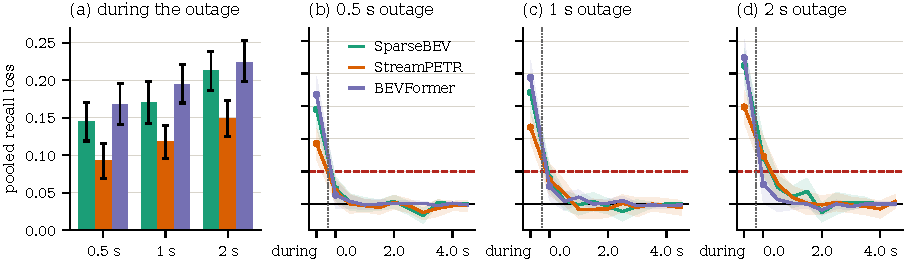
\includegraphics[width=\textwidth]{figures/fig_results.pdf}
\caption{(a) Pooled recall loss during the outage with 95\% intervals. (b)--(d) Loss during the outage and in the ten bins after restoration (axis in seconds; bands: 95\% intervals).
Dashed: the 0.05 margin; dotted: boundary between ``during'' and the post-restoration bins.}
\label{fig:results}
\end{figure*}

\subsection{Recovery}
The pooled curves (Fig.~\ref{fig:results}b--d) return to the margin almost immediately. At the first bin (0.0\,s) the loss is 0.014--0.040 for all models after 0.5\,s and 1\,s outages
and for BEVFormer after 2\,s; only SparseBEV (0.072) and StreamPETR (0.074) after 2\,s are above the margin, and both are below it from 0.5\,s. From 0.5\,s on, every pooled loss stays within $\pm0.031$,
with no step when information should leave the memory. This is notable for SparseBEV: its predictions differ from the clean run until the last black frame leaves its window (about 3.5\,s),
yet its pooled recall shows no loss at 3.0--4.0\,s (0.003, interval $-0.004$ to $0.010$, at 3.5\,s after a 2\,s outage). BEVFormer's recurrent state never returns to bit-identical predictions, but its
pooled loss is gone from the first bins. These statements concern \emph{recall at a fixed threshold}, not score or box quality. Of 90 model$\times$duration$\times$bin cells from 0.5\,s on, five have an interval excluding zero,
close to the four or five expected by chance.

Per event, 49--80\% of events with enough objects are damaged (Table~\ref{tab:main}); StreamPETR is lowest and SparseBEV and BEVFormer are not statistically distinguishable. Per-event \emph{recovery} cannot be read at face value, however:
43--77\% of damaged events have incomplete follow-up (a missing or insufficient bin, from 2\,Hz keyframes and the five-object rule), and 80, 51 and 25 of 150 events are insufficient at 0.5, 1 and 2\,s. Where follow-up is complete,
recovery is confirmed in 209 of 210 events, so the confirmed-by-4\,s fractions (0.91/0.94/0.91 at 0.5\,s down to 0.68/0.61/0.64 at 2\,s for SparseBEV/StreamPETR/BEVFormer) mostly reflect censoring.
Official whole-sequence metrics barely move after 2\,s (NDS 0.556$\to$0.552, 0.537$\to$0.534, 0.355$\to$0.352 for SparseBEV, StreamPETR, BEVFormer): a full-sequence benchmark dilutes a brief single-camera outage.

\subsection{Qualitative example}
Fig.~\ref{fig:qual} shows an event chosen by a fixed rule on event category, not by eye: SparseBEV through a 2\,s outage. The front input is black, the clean-detected objects (green) are missed (red) during the outage,
and in the first bins after restoration they are detected again; the BEV panels show the same loss and return in the ground plane.

\begin{figure*}[t]
\centering
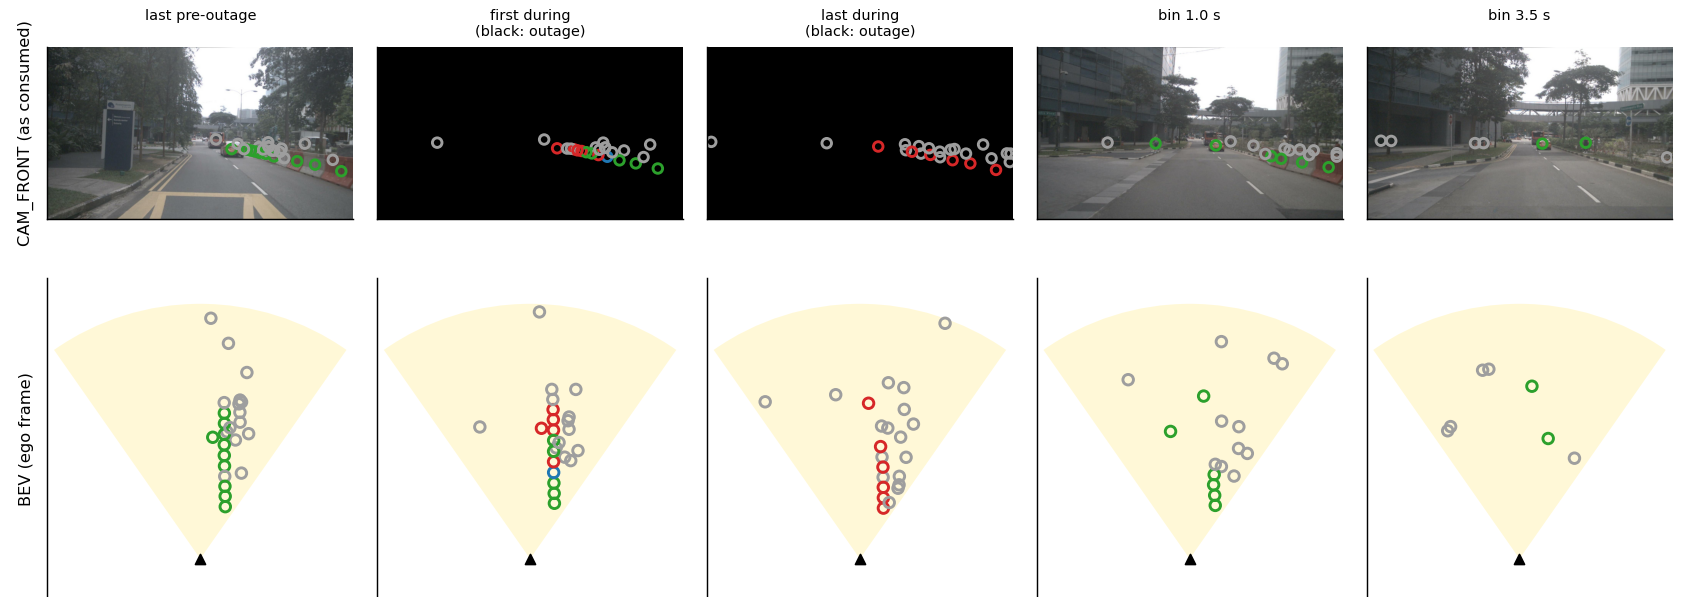
\includegraphics[width=0.78\textwidth]{figures/fig_qualitative.png}
\caption{SparseBEV, 2\,s outage, an event with recovery at the first observed bin. Top: CAM\_FRONT as consumed with projected ground truth. Bottom: BEV in the ego frame.
Green: detected in both runs; red: missed only in the outage run; grey: missed in both; blue: detected only in the outage run; orange cross: false positive.}
\label{fig:qual}
\end{figure*}

%%%%%%%%%%%%%%%%%%%%%%%%%%%%%%%%%%%%%%%%%%%%%%%%%%%%%%%%%%%%%%%%%%%%%%%%%%%%%%%%
\section{FAILURE-MODE ANALYSIS}

Pooled recovery is fast, but the aggregate hides several failure modes (Fig.~\ref{fig:failure}).

\textbf{Misses that persist after restoration.} Take objects that the clean run detects at both the last during-outage sample and the first strictly later sample with a restored front image, and that the outage run missed
during the outage; 70--95\% are detected again (Table~\ref{tab:main}). The complement, a \emph{persisting miss}, grows with outage length for all three models (Fig.~\ref{fig:failure}a): 2--12\% (SparseBEV), 5--21\% (StreamPETR) and 7--17\% (BEVFormer) of
continuing, clean-detected objects from 0.5\,s to 2\,s. StreamPETR, with the smallest loss during the outage, has the largest persisting share after 2\,s (0.21), consistent with a query memory that has lost an object's track and must
re-initialize it; we have not isolated this mechanism. Where the last ``during'' sample is also bin 0.0 by evaluation time, it cannot be compared with itself, so the next restored observation (bin 0.5\,s) is used instead.

\textbf{Precision.} At the fixed threshold, precision falls during a 2\,s outage for SparseBEV (0.940$\to$0.868) and StreamPETR (0.922$\to$0.846) but not BEVFormer (0.902$\to$0.899). StreamPETR's false positives rise (89$\to$100) while true positives fall;
SparseBEV's are unchanged (77$\to$74), so its fall is mainly missing true positives. The separate intervals overlap, so this is suggestive only.

\textbf{Which objects.} Cars dominate the absolute loss as the most numerous front-region class (2\,s: SparseBEV 0.31, StreamPETR 0.19, BEVFormer 0.35; 1,220 objects), followed by barriers and cones.
Buses lose most for StreamPETR (0.39) but on only 62 objects, and construction vehicles and trailers have fewer than 50 objects, so we flag them rather than rank them.

\textbf{Measurement artifacts.} Censoring of per-event recovery (above), and the 2\,Hz keyframes against 0.5\,s bins, which leave about five objects per bin so that ``loss $\le0.05$'' in practice means ``no object lost''.

\begin{figure*}[t]
\centering
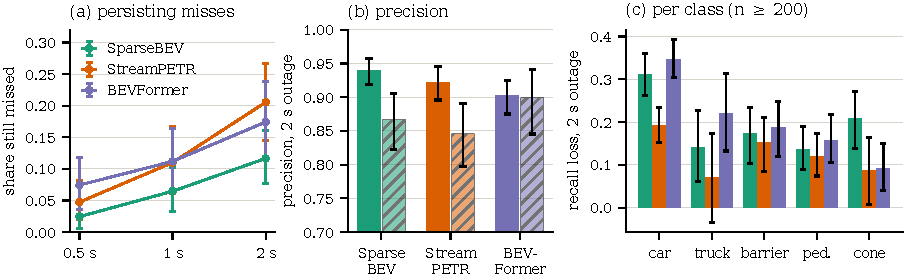
\includegraphics[width=\textwidth]{figures/fig_failure.pdf}
\caption{Failure modes. (a) Share of continuing, clean-detected objects still missed after restoration. (b) Precision for a 2\,s outage, clean (solid) and during the outage (hatched).
(c) Recall loss per class for a 2\,s outage (classes with at least 200 eligible objects). All with 95\% intervals.}
\label{fig:failure}
\end{figure*}

%%%%%%%%%%%%%%%%%%%%%%%%%%%%%%%%%%%%%%%%%%%%%%%%%%%%%%%%%%%%%%%%%%%%%%%%%%%%%%%%
\section{DISCUSSION}

\textbf{Strengths.} The protocol isolates the transition: identical physical outages across models, audited inputs, paired clean/outage runs on the same objects, operating points fixed
before validation, frozen event rules, and uncertainty that respects scene-level dependence. The controls (bit-exact repeatability, independent table rebuild, state-isolation and window tests) rule out likely
artifacts such as a stale feature cache leaking clean content into an outage run, and the treatment of censoring prevents reading unrecovered events as failures.

\textbf{Limitations.} (i) The systems differ in clean recall, thresholds, resolution, pretraining, query counts and history, so this compares complete released systems, not architectures. (ii) A black image is an idealized failure; frozen frames, noise or packet loss
may behave differently, and a frozen frame could harm a temporal model more. (iii) Pilot scenes come from the training split and may have been seen by the released models. (iv) Per-event analysis is noisy (about one sample per bin per scene, about five objects per sample).
(v) Recall at a fixed threshold ignores calibration and box quality; intervals cover scene sampling only, with one deterministic run per condition. (vi) The front region is a projection of ground-truth centers; other cameras overlap it and motion is not compensated.

\textbf{Future work.} Realistic failures (frozen frames, other cameras, simultaneous failures); denser temporal sampling with sweeps for sub-second recovery; score and box-quality recovery and calibration; a second dataset to power the per-event analysis; controlled ablations of one
temporal mechanism within a codebase (window length, memory reset on dropout) to move from description to cause; and mitigation such as detecting blank input and resetting or masking memory.

%%%%%%%%%%%%%%%%%%%%%%%%%%%%%%%%%%%%%%%%%%%%%%%%%%%%%%%%%%%%%%%%%%%%%%%%%%%%%%%%
\section{CONCLUSION AND REPRODUCIBILITY}

A front-camera outage costs three different temporal detectors 9--22 points of front-region recall, and recall returns to within five points of the clean level within one bin of restoration, with the pooled loss within 3 points of zero from 0.5\,s on,
even though SparseBEV keeps black frames in its window for about 3.5\,s. What remains is concentrated in a minority of objects that stay missed after restoration, in precision for two models, and in events whose follow-up is too short to confirm recovery.
Code, frozen declarations, the analysis notebook and figures are at \textbf{\url{https://github.com/JoonHan-v3/camera-failure-recovery}}
(\texttt{Report/report.ipynb} regenerates every figure and table from the saved results).

\begin{thebibliography}{99}

\bibitem{nuscenes} H. Caesar \emph{et al.}, ``nuScenes: A multimodal dataset for autonomous driving,'' in \emph{Proc. IEEE/CVF Conf. Computer Vision and Pattern Recognition (CVPR)}, 2020, pp. 11621--11631.

\bibitem{bevformer} Z. Li \emph{et al.}, ``BEVFormer: Learning bird's-eye-view representation from multi-camera images via spatiotemporal transformers,'' in \emph{Proc. European Conf. Computer Vision (ECCV)}, 2022.

\bibitem{streampetr} S. Wang \emph{et al.}, ``Exploring object-centric temporal modeling for efficient multi-view 3D object detection,'' in \emph{Proc. IEEE/CVF Int. Conf. Computer Vision (ICCV)}, 2023.

\bibitem{sparsebev} H. Liu \emph{et al.}, ``SparseBEV: High-performance sparse 3D object detection from multi-camera videos,'' in \emph{Proc. IEEE/CVF Int. Conf. Computer Vision (ICCV)}, 2023.

\bibitem{detr3d} Y. Wang \emph{et al.}, ``DETR3D: 3D object detection from multi-view images via 3D-to-2D queries,'' in \emph{Proc. Conf. Robot Learning (CoRL)}, 2021.

\bibitem{petr} Y. Liu \emph{et al.}, ``PETR: Position embedding transformation for multi-view 3D object detection,'' in \emph{Proc. European Conf. Computer Vision (ECCV)}, 2022.

\bibitem{bevdet4d} J. Huang and G. Huang, ``BEVDet4D: Exploit temporal cues in multi-camera 3D object detection,'' arXiv:2203.17054, 2022.

\bibitem{hendrycks2019} D. Hendrycks and T. Dietterich, ``Benchmarking neural network robustness to common corruptions and perturbations,'' in \emph{Proc. Int. Conf. Learning Representations (ICLR)}, 2019.

\bibitem{dong2023} Y. Dong \emph{et al.}, ``Benchmarking robustness of 3D object detection to common corruptions in autonomous driving,'' in \emph{Proc. IEEE/CVF Conf. Computer Vision and Pattern Recognition (CVPR)}, 2023, pp. 1022--1032.

\bibitem{xie2023} S. Xie \emph{et al.}, ``RoboBEV: Towards robust bird's eye view perception under corruptions,'' arXiv:2304.06719, 2023.

\bibitem{zhu2023} Z. Zhu \emph{et al.}, ``Understanding the robustness of 3D object detection with bird's-eye-view representations in autonomous driving,'' in \emph{Proc. IEEE/CVF Conf. Computer Vision and Pattern Recognition (CVPR)}, 2023, pp. 21600--21610.

\bibitem{ge2023} C. Ge \emph{et al.}, ``MetaBEV: Solving sensor failures for 3D detection and map segmentation,'' in \emph{Proc. IEEE/CVF Int. Conf. Computer Vision (ICCV)}, 2023, pp. 8721--8731.

\bibitem{yu2023} K. Yu \emph{et al.}, ``Benchmarking the robustness of LiDAR-camera fusion for 3D object detection,'' in \emph{Proc. IEEE/CVF Conf. Computer Vision and Pattern Recognition Workshops (CVPRW)}, 2023.

\bibitem{bevfusion} Z. Liu \emph{et al.}, ``BEVFusion: Multi-task multi-sensor fusion with unified bird's-eye view representation,'' in \emph{Proc. IEEE Int. Conf. Robotics and Automation (ICRA)}, 2023.

\end{thebibliography}

\end{document}
